\documentclass[12pt,journal,compsoc]{IEEEtran}
%\documentclass[conference]{IEEEtran}  %si es conferencia
%\documentclass[journal]{IEEEtran}     %si es un journal

\ifCLASSOPTIONcompsoc
  % IEEE Computer Society needs nocompress option
  % requires cite.sty v4.0 or later (November 2003)
  \usepackage[nocompress]{cite}
\else
  % normal IEEE
  \usepackage{cite}
\fi


\ifCLASSINFOpdf
   \usepackage[pdftex]{graphicx}
  % declare the path(s) where your graphic files are
   \graphicspath{{../pdf/}{../jpeg/}}
  % and their extensions so you won't have to specify these with
  % every instance of \includegraphics
   \DeclareGraphicsExtensions{.pdf,.jpeg,.png}
\else
  % or other class option (dvipsone, dvipdf, if not using dvips). graphicx
  % will default to the driver specified in the system graphics.cfg if no
  % driver is specified.
  \usepackage[dvips]{graphicx}
  % declare the path(s) where your graphic files are
  \graphicspath{{../eps/}}
  % and their extensions so you won't have to specify these with
  % every instance of \includegraphics
  \DeclareGraphicsExtensions{.eps}
\fi


\usepackage[utf8x]{inputenc}
\usepackage[T1]{fontenc}
\usepackage{lmodern}
\usepackage{booktabs}
\usepackage{multirow}
\usepackage[spanish,USenglish]{babel}
\usepackage[colorlinks=true,linkcolor=black,urlcolor=black,citecolor=black, urlcolor=black, filecolor=black]{hyperref}

\addto\captionsspanish{
 \def\tablename{TABLA}}


\makeatletter
\def\markboth#1#2{\def\leftmark{\@IEEEcompsoconly{\sffamily}\MakeUppercase{\protect#1}}%
\def\rightmark{\@IEEEcompsoconly{\sffamily}\MakeUppercase{\protect#2}}}
\makeatother

\begin{document}

\selectlanguage{spanish}

\title{Análisis de desempeño de algoritmos de detección de patrones de agrupamiento en Bases de Datos espacio-temporales}

\author{Sandra~Cristina~Muñoz~Castillo\IEEEauthorrefmark{1}~\IEEEauthorrefmark{2},
        Nombre~Otro~Autor\IEEEauthorrefmark{1}~\IEEEauthorrefmark{2}.
	{\IEEEauthorrefmark{1}Universidad de Nariño.}
	{\IEEEauthorrefmark{2}Grupo de Investigación Aplicada en Sistemas (GRIAS).}
\IEEEcompsocitemizethanks{\IEEEcompsocthanksitem S. Muñoz. Ingeniera de Sistemas and Magíster en 
Docencia Universitaia, Universidad de Nariño (Pasto - Colombia).
E-mail: sandramunoz@udenar.edu.co.
\IEEEcompsocthanksitem N. Apellido. Ingeniero.
E-mail: mail@udenar.edu.co. 

}

\thanks{Junio, 2014.}}

\markboth{Proyecto de Grado} 
{\MakeLowercase{\textit{et al.}}: Bare Demo of IEEEtran.cls for Computer Society Journals}

\IEEEcompsoctitleabstractindextext{%
\begin{abstract}
En esta parte se escribe el abstract en Español. Ell sid djd did djd d did didi
did did didid didid diid diid didi did
\end{abstract}

\selectlanguage{USenglish}
\begin{abstract}
Here write abstract in English. did didid didid didid didid didid didid did
didi did
 \end{abstract}

\selectlanguage{spanish}
 
\begin{IEEEkeywords}
Proyecto, escribir, latex, otras palabras, importante.
\end{IEEEkeywords}}

\maketitle


\IEEEdisplaynotcompsoctitleabstractindextext

\IEEEpeerreviewmaketitle


%%% Aqui se agregan los demas archivos para separarlos y no tener un solo archivos
%% asi es mas facil ordenar ... esto pranticamente seria el cuerpo del documento

\section{Introducción}

\IEEEPARstart{L}{os} recientes avances tecnológicos y el amplio  uso de localización por sistemas de posicionamiento global (GPS),
identificación por radio frecuencia (RFID) y tecnologías en dispositivos móviles han hecho que las bases de datos
espacio temporales recolectadas hayan incrementado con un porcentaje acelerado. Esta gran cantidad de información
ha motivado a desarrollar eficientes técnicas, para procesar consultas acerca del comportamiento de los objetos en
movimiento, como descubrir patrones de comportamiento entre las trayectorias de objetos en un periodo continuo de tiempo. 

Los métodos que existen para consulta de trayectorias se centran principalmente en responder un único rango simple
de predicado  y consultas de vecinos mas cercanos   por ejemplo:  ``encontrar todos los objetos en movimiento que se
encontraban en la zona A a las 10 de la mañana (en el pasado)'' o ``encontrar el coche que condujo tan cerca como sea posible a
la ubicación B durante el intervalo de tiempo de 10 de la mañana a 1 de la tarde''.  Recientemente, diversos estudios se han centrado
en la consulta de los patrones para la captura del comportamiento de los objetos en movimiento reflejada en colaboraciones tales como
clusters móviles \cite{jensen2007continuous} \cite{kalnis2005discovering}, consulta de convoyes 
\cite{jeung2008discovery-1} y patrones de agrupación \cite{gudmundsson2006computing} \cite{benkert2008reporting}
\cite{vieira2009line}. Estos patrones descubren grupos de objetos en movimiento que tienen una ``fuerte'' relación en
el espacio durante un tiempo determinado. La diferencia entre todos esos patrones es la forma de definir 
la relación entre los objetos en movimiento y su duración en el tiempo. 

En este artículo se enfocará en el descubrimiento de patrones de agrupación, conocidos como ``flocks'', entre los objetos 
en movimiento de acuerdo
a las características de los objetos de estudio (animales, peatones, vehículos o fenómenos naturales), como 
interactúan entre si y como se mueven juntos \cite{laube2005finding} \cite{uno2005lcm}.  \cite{vieira2009line} 
define patrones de agrupamiento como el problema de identificar todos los grupos de trayectorias que permanecen
``juntas'' por la duración de un intervalo de tiempo dado. Consideramos que los objetos en movimiento están suficientemente
cerca si existe un disco con un
radio dado que cubre todos los objetos que se mueven en el patrón (Figura~\ref{fig:flockexample}). Una trayectoria satisface el 
patrón anterior, siempre y cuando suficientes trayectorias están contenidos dentro del disco para el intervalo de
tiempo especificado, es decir, la respuesta se basa no sólo en el comportamiento de una trayectoria dada, sino
también en los más cercanos a él. El enfoque actual para descubrir patrones de agrupación de movimiento consiste
en encontrar un conjunto adecuado de discos en cada instante de tiempo y luego la fusión de los resultados de un 
instante de tiempo a otro. Como consecuencia, el rendimiento y el número de patrones final depende del número
de los discos y cómo estos se combinan.

En el ejemplo de la Figura~\ref{fig:flockexample} se muestra un patrón de agrupamiento el cual contienen tres 
trayectorias {T1, T2, T3}
que están dentro de un disco en tres instantes de tiempo consecutivos. Los discos se pueden
mover libremente en el espacio bidimensional con el fin de acomodar los tres objetos en movimiento  y su centro no
tiene por que ser cualquiera de las localizaciones  de los objetos en movimiento. Esto hace que el
descubrimiento de agrupación de patrones sea mucho más complicada  porque hay un número infinito de posibles
colocaciones del disco en cualquier instante de tiempo y el posible número de combinaciones convierten
al problema en un problema NP-complejo.

La implementación de este algoritmo tiene diversas aplicaciones tales como: sistemas  integrados  de  transporte,
seguridad  y  monitoreo, seguimiento  a  grupos  de  animales  y  fenómenos  naturales,  encontrando  así  una
alternativa  diferente  para  solucionar  los  problemas  en  el  mundo,  analizando  como  se mueven  los  objetos
en  la  tierra  y  cuales  son  los  patrones  de  comportamiento  que existen entre si. 

En este artículo se muestra una comparación entre dos algoritmos, el propuesto por \cite{vieira2009line} y 
\cite{romero2011mining}, con el fin de identificar los problemas asociados a su rendimiento, y probando
estos algoritmos en distintos conjuntos de datos.


\begin{figure}
  \centering
  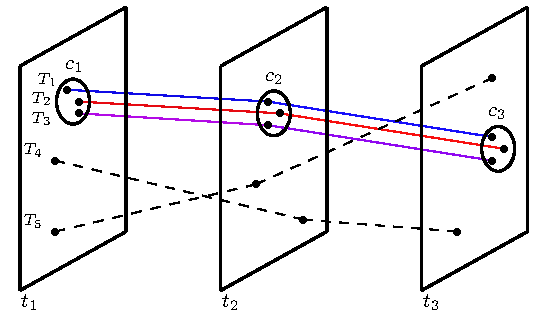
\includegraphics[scale=0.8]{pictures/flock_example}
  \caption{Ejemplo de patrones de agrupamiento} %(\cite{vieira2009line}).}
  \label{fig:flockexample}
\end{figure}
\section{Trabajos Relacionados}

Las capacidad de recolectar datos de objetos en movimiento ha ido aumentando rápidamente y el interés de consulta
de patrones que describen el comportamiento colectivo también ha aumentado. \cite{vieira2009line} enumera tres grupos de patrones
``colectivos'' en bases de datos de objetos en movimiento: clústers móviles, consulta de convoyes y patrones de agrupación.

Los clústers móviles \cite{jensen2007continuous} \cite{kalnis2005discovering} \cite{li2008mining} 
y  consultas de convoyes  \cite{jeung2008discovery-1} \cite{jeung2008convoy}, tienen en común que se basan en algoritmos
de clústering, principalmente en algoritmos basados en densidad como el algoritmo DBSCAN\cite{ester1996density}.

Los clústers móviles se definen entre dos instantes de tiempo consecutivos.
Los clústers  se pueden unir sólo si el número de objetos comunes entre ellos están por encima del parámetro predefinido.
Un clúster es reportado si no hay otro nuevo clúster que pueda ser unido a este. Este proceso se aplica cada vez para 
todos los instantes de tiempo en el conjunto de datos. 

Las consultas de convoyes se definen como un clúster denso de trayectorias que permanecen juntas al menos por un por
un tiempo continuo predefinido. 

Las principales diferencias entre las dos técnicas son la forma en que se unen los grupos  entre dos intervalos
consecutivos de tiempo y el uso de un parámetro adicional para especificar un tiempo mínimo de duración. Aunque
estos métodos están estrechamente relacionados con los patrones de agrupamiento, ninguno de ellos asume una  forma predefinida.

Previos trabajos de detección de patrones de agrupamiento móviles son descritos por \cite{ gudmundsson2006computing}
y \cite{benkert2008reporting}. Ellos introducen
el uso de discos con un radio predefinido para identificar  grupos de trayectorias que se mueven juntos en la misma
dirección, todas las trayectorias que se encuentran dentro del disco en un instante  de tiempo particular se 
considera un patrón candidato. La principal limitación de este proceso es que hay un número infinito de posibles
ubicaciones del disco en cualquier instante de tiempo. En efecto, \cite{gudmundsson2006computing} han demostrado
que el descubrimiento de agrupaciones fijas, donde los patrones de las mismas entidades permanecen juntas durante 
todo el intervalo, es un problema NP-complejo. 

\cite{vieira2009line} on  los  primeros  en  presentar  una  solución  exacta  para  reportar  patrones  de
agrupación en tiempo polinomial, y también pueden trabajar efectivamente en tiempo
real. Su trabajo revela que el tiempo de solución polinomial se puede encontrar a través
de  la  identificación  de  un  número  discreto  de  ubicaciones  para  colocar  el  centro  del
disco.  Los  autores  proponen  el  altoritmo  BFE  (Basic  Flock  Evaluation)  basado  en  el
tiempo de unión y combinación de los discos. La idea principal de este algoritmo es
primero  encontrar  el  número  de  discos  válidos  en  cada  instante  de  tiempo  y  luego
combinarlos  uno  a  uno  entre  tiempos  adyacentes. Adicionalmente  se  proponen  otros
cuatro  algoritmos  basados  en  métodos  heurísticos,  para  reducir  el  número  total  de
candidatos  a  ser  combinados  y,  por  lo  tanto,  el  costo  global  computacional  del
algoritmo  BFE.  Sin  embargo,  el pseudocódigo y  los  resultados  experimentales
muestran todavía una alta complejidad computacional, largos tiempos de respuesta y un
gran número de patrones que hace difícil su interpretación.


\cite{romero2011mining} propone  una  metodología  que  permite  identificar  patrones  de  agrupamiento  en
movimiento utilizando tradicionales y potentes algoritmos de minería de datos usando
reglas de asociación, el cual fue comparado con BFE demostrando un alto rendimiento
con conjuntos de datos sintéticos, aunque con conjuntos de datos reales el tiempo de
respuesta siguió siendo eficiente pero similar a BFE. Este algoritmo trata el conjunto de
trayectorios como una base de datos transaccional al convertir cada trayectoria, que se
define  como  un  conjunto  de  lugares  visitados,  en  una  transacción,  definida  como  un
conjunto  ítems.  De  esta  manera,  es  posible  aplicar  cualquier  algoritmo  de  reglas  de
asociación y encontrar patrones frecuentes sobre el conjunto dado.

\section{Implementación}

Se implementaron los algorítmos BFE y LCMFLOCK basados en el pseudo-código publicado por \cite{vieira2009line}  y \cite{romero2011mining} respectivamente,
usando python version 3.

\subsection{BFE}

Este algoritmo se divide en dos partes: la primera parte, encontrar los discos que contienen el mayor número de puntos
dado un radio ($\epsilon$) y un número mínimo de puntos ($\mu$) dentro de ese radio para instante de tiempo. La segunda parte: encontrar
el número de puntos que se mueven juntos (flocks) en un tiempo mímimo ($\delta$).

Para la primera parte es necesarios la utilización tanto de diccionarios de datos como
estructuras kd-tree para la búsqueda del vecino más cercano, en esta implementación se uso la clase scipy.spatial.cKDTree de
SciPy \footnote{Scipy es un ecosistema basado en Python, software de código abierto para las matemáticas, la ciencia y la ingeniería.
\url{http://www.scipy.org/}} la cual proporciona  un índice dentro de un conjunto de puntos k-dimensionales que se pueden utilizar
para buscar rápidamente los vecinos más cercanos de cualquier punto.

\subsection{LCMFLOCK}

Este algoritmo usa la primera parte del algoritmo de BFE que es encontrar los discos maximos, en la segunda parte para abordar el problema
de combinatoria utiliza un enfonque de patron frecuente de mineria, en el cual se contruyo un diccionario de datos asociando la localizacion 
de los puntos de cada trayectoria con su respectivo disco en orden para generar una version transaccional del conjunto de datos. Este conjunto
es pasado como parametro junto con el umbral mínimo de soporte (min\_sup), para el algoritmo de LCM, disponible para descargar en \cite{FIMIHomep},
 están disponibles dos variantes del programa; LCM\_max y LCM\_closed los cuales recuperarán el conjunto máximo o cerrado de los patrones de 
 frecuencia, dependiendo del caso. La salida M es un archivo de texto sin formato, donde cada línea es un patrón máxima que 
 contiene un conjunto de ID's de discos separados por espacios.
\section{Experimentación Computacional}

Los resultados fueron producidos usando conjuntos de datos sintéticos y reales en una máqina
Dell OPTIPLEX 7010 con procesador Intel\textregistered Core\texttrademark  i7-3770 CPU de 3.40GHz x 8,
16 GB de RAM y 1TB 7200 RPM de Disco Duro, corriendo Ubuntu con linux 3.5. Para todos los casos se usaron
los algoritmos implementados en python version 3.

\subsection{San Joaquin}

Un grupo de conjuntos de datos sintéticos fueron creados usando un modelo para la generación de objetos en movimiento, como se describe en \cite{brinkhoff2002framework}.
Dos conjuntos de datos sintéticos fueron creados usando la red de San Joaquín proporcionada en el sitio web del generador basado en red \cite{Brin:2010:Online}.
El primer conjunto de datos recoge 992140 lugares simulados para 25.000 objetos en movimiento durante 60 instantes de tiempo. El segundo recoge 50.000 trayectorias
de 2.014.346 de puntos durante 55 instantes de tiempo. La Table~\ref{tab:datasets} resume la información principal. Es importante aclarar que el tamaño de la trayectoria se refiere al
número promedio de ubicaciones de puntos e intervalos de tiempo en lugar de a la longitud espacial media.


\begin{table}
\caption{Conjunto de datos sintéticos}
\label{tab:datasets}
\centering
\scalebox{0.8}{
\begin{tabular}{c c r r c}
\toprule
\multirow{2}{*}{Dataset}& \multirow{2}{*}{Network}& \multicolumn{1}{c}{Number of}& Number of  & Trajectory\\
                        &                         & Trajectories & \multicolumn{1}{c}{Points} & size (avg)\\
\midrule
SJ25KT60  & San Joaquin & 25000 & 992140  & 40\\
SJ50KT55  & San Joaquin & 50000 & 2014346 & 37\\
TAPAS Cologne  & Cologne, Germany & 49225 & 1813454 & 37\\
Original\_Beijing   & Beijing, China   & 23800 & 1207110 & 50\\
Alternative\_Beijing   & Beijing, China   & 18216 & 760814 & 42\\
\bottomrule
\end{tabular}}
\end{table}

\begin{figure}
  \centering
  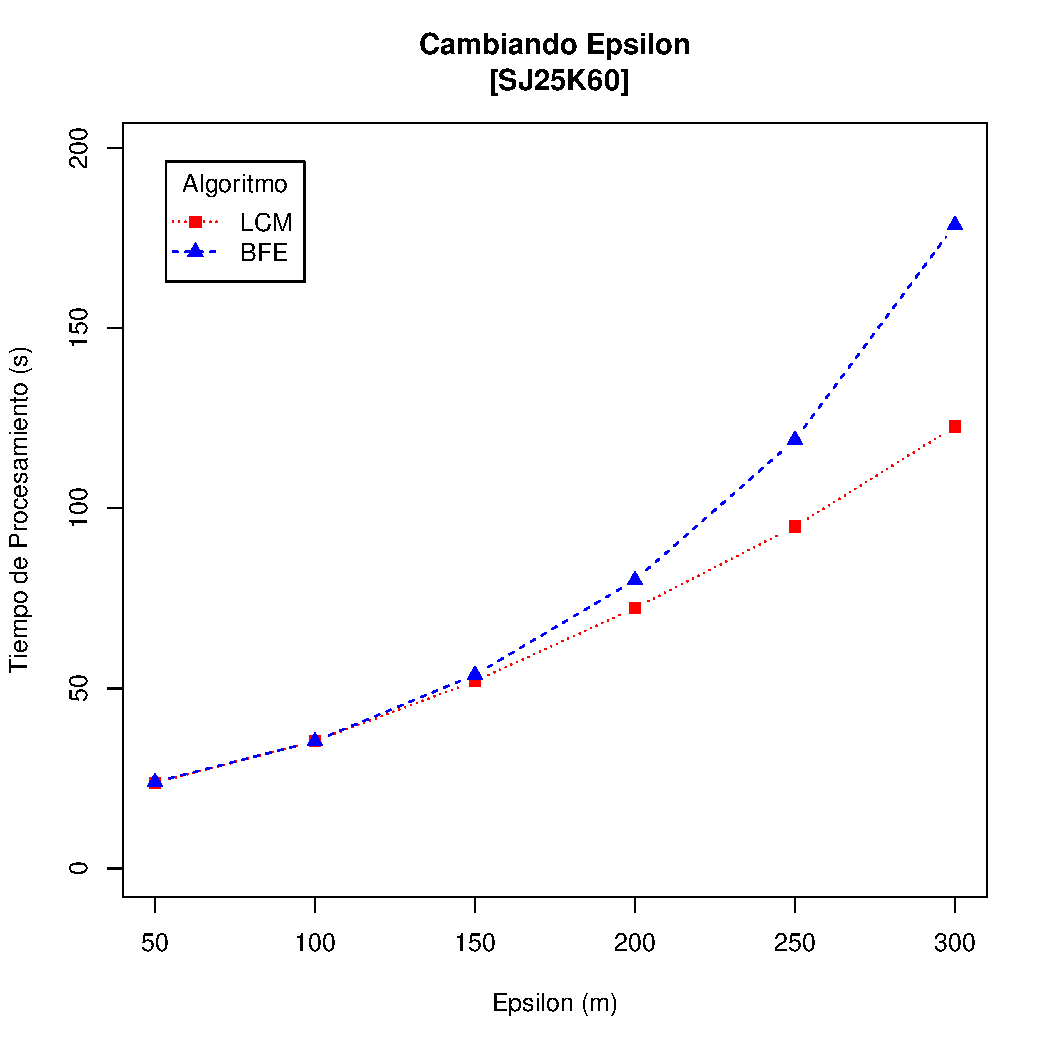
\includegraphics[scale=0.4]{pictures/SJ25K60.pdf}
  \caption{Caso de Prueba: SJ25K60}
  \label{fig:SJ25K60}
\end{figure}

\begin{figure}
  \centering
  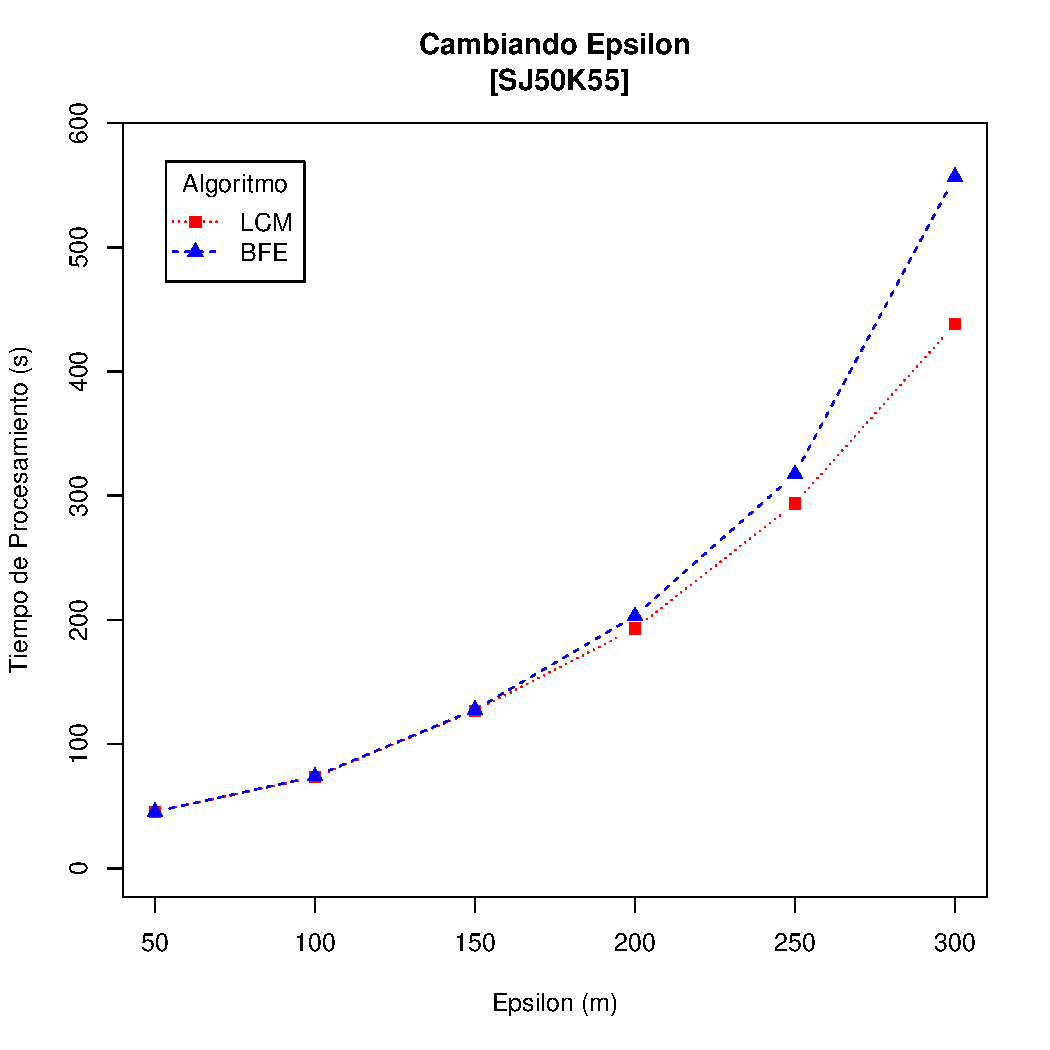
\includegraphics[scale=0.4]{pictures/SJ50K55.pdf}
  \caption{Caso de Prueba: SJ50K55}
  \label{fig:SJ50K55}
\end{figure}

\subsection{TAPAS Cologne}

Este conjunto de datos sintético se preparó utilizando el escenario TAPAS Cologne \cite{varschen2006mikroskopische}
en SUMO \cite{krajzewicz2002sumo}, un reconocido simulador de tráfico para la movilidad urbana. El escenario de simulación 
TAPAS Colonia describe el tráfico dentro de la ciudad de Cologne (Alemania) durante un día entero. La principal ventaja de 
este conjunto de datos es que sus trayectorias no se generan aleatoriamente. Los datos de la demanda original, se deriva de TAPAS, 
un sistema que calcula el deseo de movilidad para una población de la zona generada con base en la información sobre los hábitos de viaje 
de los alemanes y en la información sobre la infraestructura de la zona en que viven \cite{MiD2002}. El conjunto de datos original 
es enorme por lo que sólo una esta disponible al público la versión de 2 horas \cite{TAPASCologne}. Debido a la memoria constriñe 
las trayectorias más cortas que se podaron 20 minutos. El último conjunto de datos recoge 49.225 trayectorias y más 
de 1,8 millones de puntos. La Tabla~\ref{tab:datasets} describe los detalles sobre el conjunto de datos.

\subsection{Movimiento de peatones en Beijing}

Este conjunto de datos reales recopila información de movimiento de un grupo de personas en todo 
el área metropolitana de Beijing, China, el uso de un conjunto de datos de la trayectoria GPS proporcionado por \cite{GeoLife}. 
El conjunto de datos se recogieron durante el proyecto Geolife por 165 usuarios anónimos en un período de dos años entre abril de 2007 y agosto de 2009. Ubicaciones eran 
grabada por diferentes registradores GPS o Smartphones y la mayoría de ellos presentan una frecuencia de muestreo alta. 
La región alrededor de la ``5th Ring Road'' en el área metropolitana de Beijing mostró la 
mayor concentración de trayectorias. Esto fue usado para generar un conjunto de datos de muestra. Cada trayectoria 
fue interpolada por minuto (un punto por minuto) y saltos de 20 minutos o más 
sin señal se utilizaron para marcar una nueva trayectoria. Por último, el conjunto de datos recoge más 
de 1,2 millones de ubicaciones de puntos y 23.800 trayectorias. Sin embargo, como este conjunto de datos seguimiento poca cantidad de
entidades en movimiento (165 usuarios) en una ventana de tiempo (más de 2 años) no hay mucho trayectorias fueron sucediendo al mismo tiempo. Para probar
la escalabilidad se decidió crear un conjunto de datos alternativo basado en las trayectorias reales, pero todos ellos a partir de la mismo tiempo. Una 
vez más, para la memoria limita las trayectorias más cortas que 10 minutos y más de 3 horas se podaron. El conjunto de datos alternativa almacena 760.814 
ubicaciones de los puntos y 18.216 trayectorias reales que ocurren juntos. La Tabla~\ref{tab:datasets} resume los detalles para ambos conjuntos de datos.


\begin{figure}
  \centering
  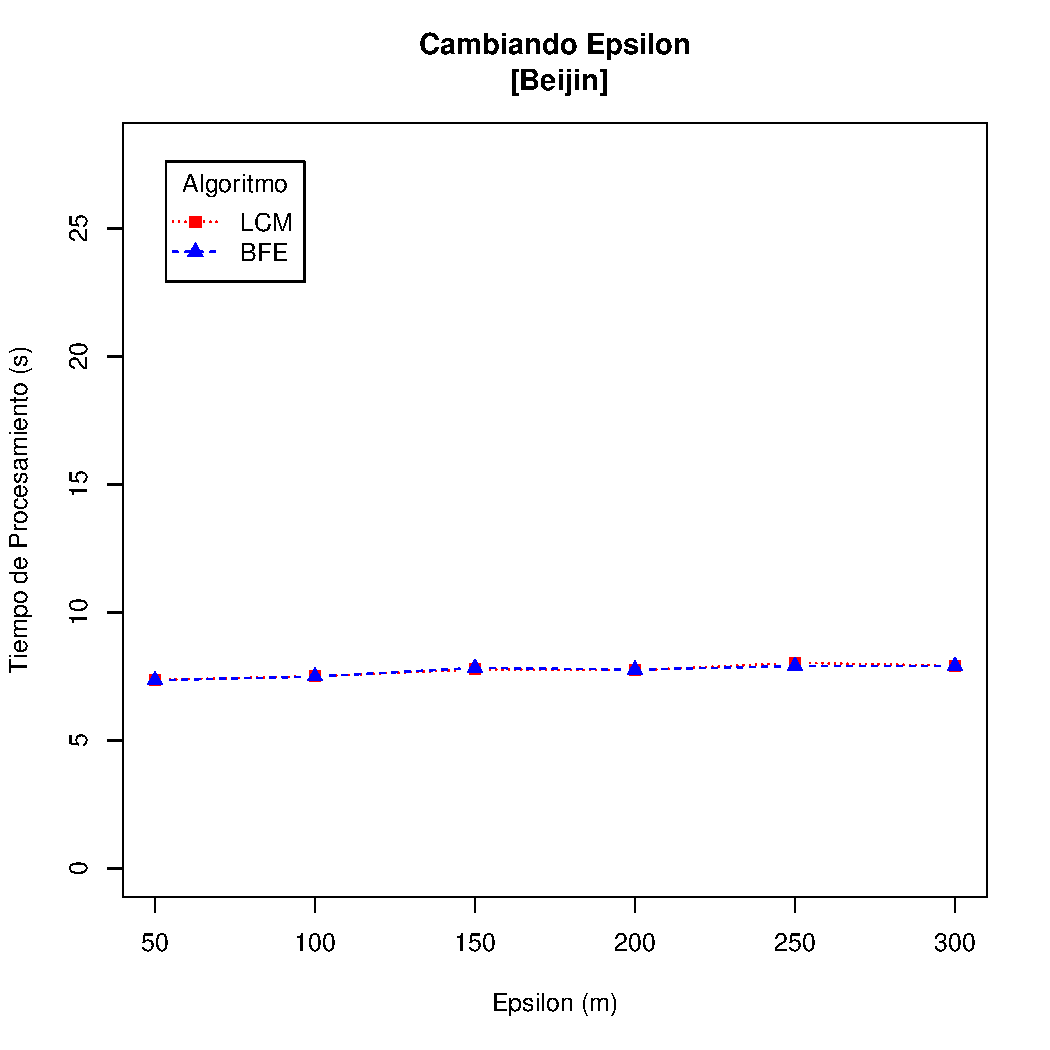
\includegraphics[scale=0.4]{pictures/Beijin.pdf}
  \caption{Caso de Prueba: Beijin}
  \label{fig:Beijin}
\end{figure}

\section{Conclusiónes}

Aquí las conclusiones


%\appendices
%\section{Repositorio}
%El código fuente y conjunto de datos se encuentran en el repositorio de github.


\ifCLASSOPTIONcompsoc
  % The Computer Society usually uses the plural form
  \section*{Agradecimientos}
\else
  % regular IEEE prefers the singular form
  \section*{Agradecimiento}
\fi


Aquí se agredece a la facultad y al programa y la universidad ... si es 
investigación a quien la financio 


% Can use something like this to put references on a page
% by themselves when using endfloat and the captionsoff option.
\ifCLASSOPTIONcaptionsoff
  \newpage
\fi


\bibliographystyle{IEEEtran}

\bibliography{IEEEabrv,bibliography} 

%% el archivo bibliography.bib es donde tiene toda la bibliografia.
%% cuando busques bibliografia por eso busca bibtex y eso se copia al archivo.

\end{document}
